\باب{درجہ اول سادہ تفرقی مساوات}
عموماً طبعی تعلقات کو تفرقی مساوات کی صورت میں لکھا جا سکتا ہے۔اسی طرح عموماً انجنیئرنگ مسائل تفرقی مساوات کی صورت میں پیش آتے ہیں۔اسی لئے  اس کتاب کی ابتدا تفرقی مساوات اور ان کے حل سے کی جاتی ہے۔

\اصطلاح{سادہ تفرقی مساوات}\فرہنگ{تفرقی!سادہ مساوات}\حاشیہب{ordinary differential equation}\فرہنگ{differential!ordinary equation} سے مراد ایسی تفرقی مساوات ہے جس میں ایک عدد آزاد متغیرہ پایا جاتا ہو۔اس کے برعکس \اصطلاح{جزوی تفرقی مساوات}\فرہنگ{تفرقی!جزوی مساوات}\حاشیہب{partial differential equation}\فرہنگ{differential!partial equation} ایک سے زائد آزاد متغیرات پر منحصر ہوتی ہے۔جزوی تفرقی مساوات کا حل نسبتاً مشکل ثابت ہوتا ہے۔

کسی بھی حقیقی صورت حال یا مشاہدے کی نقشہ کشی کرتے ہوئے  اس کا \اصطلاح{ریاضی نمونہ}\فرہنگ{نمونہ!ریاضی}\حاشیہب{mathematical model}\فرہنگ{model!mathematical} حاصل کیا جا سکتا ہے۔سائنس کے مختلف میدان مثلاً انجنیئرنگ، طبیعیات، علم کیمیا، حیاتیات، کمپیوٹر وغیرہ میں درپیش مسائل کی صحیح تفرقی مساوات کا حصول اور ان کے حل پر تفصیلاً غور کیا جائے گا۔

باب-20 میں سادہ تفرقی مساوات کا حل بذریعہ کمپیوٹر  پیش کیا جائے گا۔یہ باب بقایا کتاب سے مکمل طور پر علیحدہ رکھا گیا ہے۔ یوں کتاب کے پہلے  دو باب کے بعد باب-20 پڑھا جا سکتا ہے۔

پہلے باب کا آغاز  درجہ اول کے سادہ تفرقی مساوات کے حصول، مساوات کے حل اور حل کی تشریح  سے کیا جاتا ہے۔پہلے درجے کی سادہ تفرقی مساوات میں صرف ایک عدد نا معلوم تفاعل کا ایک درجی تفرق پایا جاتا ہے۔ایسی مساوات میں ایک سے زیادہ درجے کا تفرق نہیں پایا جاتا۔نا معلوم تفاعل کو \عددی{y(t)} یا \عددی{y(x)} سے ظاہر کیا جائے گا جہاں غیر تابع متغیرہ  \عددی{t}  وقت کو ظاہر کرتی ہے۔باب کے اختتام میں تفرقی مساوات کے حل کی \اصطلاح{وجودیت}\فرہنگ{وجودیت}\حاشیہب{existence}\فرہنگ{existence}  اور \اصطلاح{یکتائی}\فرہنگ{یکتائی}\حاشیہب{uniqueness}\فرہنگ{uniqueness} پر غور کیا جائے گا۔

تفرقی مساوات سمجھنے کی خاطر ضروری ہے کہ انہیں کاغذ اور قلم سے حل کیا جائے البتہ کمپیوٹر کی مدد سے آپ حاصل جواب کی درستگی دیکھنا چاہیں تو اس میں کوئی حرج نہیں ہے۔

\حصہ{نمونہ کشی}
شکل \حوالہ{شکل_سادہ_اول_نمونہ_کشی_عمل_الف} کو دیکھیے۔ انجنیئرنگ مسئلے کا حل تلاش کرنے میں پہلا قدم مسئلے کو مساوات کی صورت میں بیان کرنا ہے۔مسئلے کو مختلف متغیرات اور تفاعل کے تعلقات کی صورت میں لکھا جاتا ہے۔اس مساوات کو \اصطلاح{ریاضی نمونہ}\فرہنگ{نمونہ!ریاضی}\حاشیہب{mathematical model}\فرہنگ{model!mathematical} کہا جاتا ہے۔ریاضی نمونے کا حصول، نمونے کا ریاضیاتی حل اور حل کی تشریح کے عمل کو \اصطلاح{نمونہ کشی}\فرہنگ{نمونہ کشی}\حاشیہب{modeling}\فرہنگ{modeling} کہا جاتا ہے۔
\begin{figure}
\centering
\begin{tikzpicture}[node distance = 2.5cm, auto]
\tikzstyle{block} = [rectangle, draw, 
    text width=5em, text centered, rounded corners, minimum height=4em]
 \node [block] (ka) {\RL{طبعی نظام}};
\node[block,right of=ka](kb){\RL{ریاضی نمونہ}};
\node[block,right of=kb](kc){\RL{ریاضی حل}};
\node[block,right of=kc](kd){\RL{تشریح}};
\draw[-latex] (ka)--(kb);
\draw[-latex] (kb)--(kc);
\draw[-latex] (kc)--(kd);
\end{tikzpicture}
\caption{نمونہ کشی، حل اور تشریح۔}
\label{شکل_سادہ_اول_نمونہ_کشی_عمل_الف}
\end{figure}
نمونہ کشی کی صلاحیت تجربے سے حاصل ہوتی ہے۔کسی بھی نمونہ کی حل میں کمپیوٹر مدد کر سکتا ہے البتہ نمونہ کشی میں کمپیوٹر عموماً کوئی مدد فراہم نہیں کر پاتا۔

عموماً طبعی مقدار مثلاً اسراع اور رفتار درحقیقت میں تفرق کو ظاہر کرتے ہیں لہٰذا بیشتر ریاضی نمونے مختلف متغیرات اور تفاعل کے تفرق پر مشتمل ہوتے ہیں جنہیں \اصطلاح{تفرقی مساوات}\فرہنگ{تفرقی مساوات}\حاشیہب{differential equation}\فرہنگ{differential equation} کہا جاتا ہے۔تفرقی مساوات کے حل سے مراد ایسا تفاعل ہے جو اس تفرقی مساوات پر پورا اترتا ہو۔تفرقی مساوات کا حل جانتے ہوئے مساوات میں موجود متغیرات اور تفاعل کے ترسیم کھینچے جا سکتا ہے اور ان پر غور کیا جا سکتا ہے۔تفرقی مساوات پر غور سے پہلے چند بنیادی تصورات تشکیل دیتے ہیں جو اس باب میں استعمال کی جائیں گی۔


\اصطلاح{سادہ تفرقی مساوات}\فرہنگ{تفرقی!سادہ مساوات} سے مراد ایسی مساوات ہے جس میں نا معلوم تفاعل کی ایک درجی یا بلند درجی تفرق پائے جاتے ہوں۔نا معلوم تفاعل کو \عددی{y(t)} یا \عددی{y(x)} سے ظاہر کیا جائے گا جہاں غیر تابع متغیر \عددی{t} وقت کو ظاہر کرتی ہے۔اس مساوات میں نا معلوم تفاعل \عددی{y} اور غیر تابع متغیرہ \عددی{x} (یا \عددی{t}) کے تفاعل بھی پائے جا سکتے ہیں۔درج ذیل چند سادہ تفرقی مساوات ہیں
\begin{align}
&y'=\sin x \label{مساوات_سادہ_اول_اول_درجہ}\\
&y'+\frac{6}{7}y=4e^{-\frac{3}{2}x} \label{مساوات_سادہ_اول_دوسرا_درجہ}\\
&y'\!'\!'+2y'-11y'^2=0 \label{مساوات_سادہ_اول_تیسرا_درجہ}
\end{align}
جہاں \عددی{y'=\tfrac{\dif y}{\dif x}}، \عددی{y'\!'=\tfrac{\dif{\,^2} y}{\dif x^2}}، وغیرہ ہیں۔

دو یا دو سے زیادہ  متغیرات کے تابع تفاعل کے تفرق پر مشتمل مساوات کو جزوی تفرقی مساوات کہتے ہیں۔ان کا حل سادہ تفرقی مساوات  سے زیادہ مشکل ثابت ہوتا ہے۔جزوی تفرقی مساوات پر بعد میں غور کیا جائے گا۔غیر تابع متغیرات \عددی{x} اور \عددی{y} پر منحصر تابع تفاعل \عددی{u(x,y)} کی جزوی تفرقی مساوات کی مثال درج ذیل ہے۔
\begin{align}
\frac{\partial^2 u}{\partial x^2}+\frac{\partial^2 u}{\partial y^2}=u
\end{align}
\عددی{n} درجی تفرقی مساوات سے مراد ایسی مساوات ہے جس میں نا معلوم تفاعل \عددی{y} کی بلند تر تفرق \عددی{n} درجے کی ہو۔یوں مساوات \حوالہ{مساوات_سادہ_اول_اول_درجہ} اول درجے کی مساوات ہے، مساوات \حوالہ{مساوات_سادہ_اول_دوسرا_درجہ} دوسرے درجے  جبکہ مساوات \حوالہ{مساوات_سادہ_اول_تیسرا_درجہ} تیسرے درجے کی مساوات ہے۔

اس باب میں پہلے درجے کی سادہ تفرقی مساوات پر غور کیا جائے گا۔ایسی مساوات میں اکائی درجہ تفرق \عددی{y'} کے علاوہ نا معلوم تفاعل \عددی{y} اور غیر تابع متغیرہ کا کوئی بھی تفاعل  پایا جا سکتا ہے۔ایک درجے کی سادہ تفرقی مساوات کو
\begin{align}\label{مساوات_سادہ_اول_درجہ_خفی}
F(y,y',x)=0
\end{align}
یا 
\begin{align}\label{مساوات_سادہ_اول_درجہ_صریح}
y'=f(x,y)
\end{align}
لکھا جا سکتا ہے۔مساوات \حوالہ{مساوات_سادہ_اول_درجہ_خفی} \اصطلاح{خفی}\فرہنگ{خفی}\حاشیہب{implicit}\فرہنگ{implicit}  صورت کہلاتی ہے جبکہ مساوات \حوالہ{مساوات_سادہ_اول_درجہ_صریح} \اصطلاح{صریح}\فرہنگ{صریح}\حاشیہب{explicit}\فرہنگ{explicit} صورت کہلاتی ہے۔یوں خفی مساوات\عددی{x^{2}y'-2y^3=0} کی صریح صورت \عددی{y'=2\tfrac{y^3}{x^2}} ہے۔

\حصہء{حل کا تصور}
ایک تفاعل
\begin{align}
y=h(x)
\end{align}
جو \اصطلاح{کھلے وقفہ}\فرہنگ{کھلا!وقفہ}\فرہنگ{وقفہ!کھلا}\حاشیہب{open interval}\فرہنگ{open!interval}\فرہنگ{interval!open} \عددی{a\le x \le b} پر \اصطلاح{معین}\فرہنگ{معین}\حاشیہب{defined}\فرہنگ{defined} ہو اور پورے وقفے پر اس کا تفرق پایا جاتا ہو، اس صورت مساوات \حوالہ{مساوات_سادہ_اول_درجہ_خفی} کا حل ہو گا جب \عددی{h(x)} اور \عددی{h'(x)} کو  مساوات \حوالہ{مساوات_سادہ_اول_درجہ_خفی} میں بالترتیب \عددی{y(x)} اور \عددی{y'(x)} کی جگہ پر کرنے سے مساوات کے دونوں اطراف برابر ہوں۔تفاعل \عددی{h(x)} کا خط \اصطلاح{منحنی حل}\فرہنگ{منحنی حل}\حاشیہب{solution curve}\فرہنگ{solution curve} کہلائے گا۔

یہاں کھلے وقفے سے مراد ایسا وقفہ ہے جس کے آخری سر \عددی{a} اور \عددی{b} وقفے کا حصہ نہ ہوں۔کھلا وقفہ لامتناہی ہو سکتا ہے مثلاً \عددی{-\infty \le x \le b} یا \عددی{a \le x \le \infty} اور  یا \عددی{-\infty \le x \le \infty} یعنی حقیقی محور۔
%====================
\ابتدا{مثال}
ثابت کریں کہ وقفہ \عددی{-\infty \le x \le \infty} پر تفاعل \عددی{y=cx} تفرقی مساوات \عددی{y=y' x} کا حل ہے جہاں \عددی{c} ایک \اصطلاح{اختیاری مستقل}\فرہنگ{اختیاری!مستقل}\فرہنگ{مستقل!اختیاری}\حاشیہب{arbitrary constant}\فرہنگ{arbitrary constant} ہے۔

حل:پورے وقفے پر \عددی{y=cx} معین ہے۔اسی طرح اس کا تفرق \عددی{y'=c} بھی پورے وقفے پر پایا جاتا ہے۔ان بنیادی شرائط پر پورا اترنے کے بعد تفاعل اور تفاعل کے تفرق کو دیے گئے تفرقی مساوات میں پر کرتے ہیں۔
\begin{align*}
y&=cx\\
(cx)&=(c)x
\end{align*}
مساوات کے دونوں اطراف برابر ہیں لہٰذا \عددی{y=cx} دیے گئے تفرقی مساوات کا حل ہے۔
\انتہا{مثال}
%=======================
\ابتدا{مثال}\شناخت{مثال_تفرقی_اول_حل_نسل_الف}
حل بذریعہ تکمل: مساوات \عددی{y'=\cos t} کا حل بذریعہ تکمل حاصل کیا جا سکتا ہے یعنی \عددی{y=\int \cos t} جس سے \عددی{y=c-\sin t} حاصل ہوتا ہے جو \اصطلاح{نسلِ حل}\فرہنگ{نسل!حل}\فرہنگ{حل!نسل}\حاشیہب{solution family}\فرہنگ{solution!family} ہے۔ حاصل حل میں \عددی{c} اختیاری مستقل ہے۔اختیاری مستقل کی ہر انفرادی قیمت تفرقی مساوات کا ایک منفرد حل دیتا ہے۔یوں \عددی{c=3.24} پر کرتے ہوئے \عددی{y=3.24-\sin t} حل حاصل ہوتا ہے۔شکل \حوالہ{شکل_مثال_تفرقی_اول_حل_نسل_الف} میں \عددی{c=-6,-3,0,3,6} سے حاصل حل دکھائے گئے ہیں۔
\begin{figure}
\centering
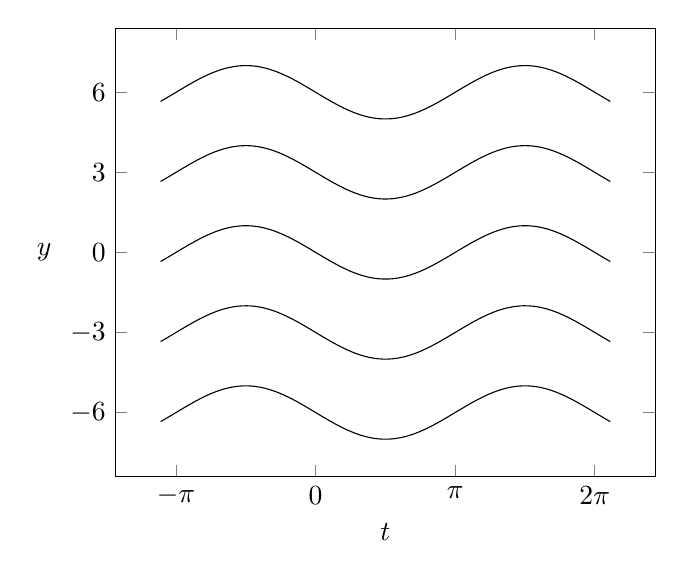
\begin{tikzpicture}
\begin{axis}[xlabel={$t$},ylabel={$y$},ylabel style={rotate=-90},xtick={-180,0,180,360},xticklabels={$-\pi$,$0$,$\pi$,$2\pi$},ytick={-6,-3,0,3,6},yticklabels={$-6$,$-3$,$0$,$3$,$6$}]
\addplot[domain=-200:380,samples=100] {6-sin(x)};
\addplot[domain=-200:380,samples=100] {3-sin(x)};
\addplot[domain=-200:380,samples=100] {-sin(x)};
\addplot[domain=-200:380,samples=100] {-3-sin(x)};
\addplot[domain=-200:380,samples=100] {-6-sin(x)};
\end{axis}
\end{tikzpicture}
\caption{مثال \حوالہ{مثال_تفرقی_اول_حل_نسل_الف} کے خط۔}
\label{شکل_مثال_تفرقی_اول_حل_نسل_الف}
\end{figure}
\انتہا{مثال}
%=========================
\ابتدا{مثال}\شناخت{مثال_تفرقی_اول_مالتھس_الف}
قوت نمائی تفاعل \عددی{y=ce^{kt}} کے تفرق سے درج ذیل تفرقی مساوات حاصل ہوتی ہے۔
\begin{align*}
y'=\frac{\dif y}{\dif t}=k ce^{kt}=ky
\end{align*}
یوں \عددی{y'=ky} تفرقی مساوات کا حل \عددی{y=ce^{kt}} ہے۔مثبت \عددی{k} کی صورت میں \عددی{y=ce^{kt}} قوت نمائی اضافے کی نمونہ کشی کرتی ہے۔جرسوموں کی تعداد اسی کلیے کے تحت بڑھتی ہے۔ وسیع رقبے کے ملک میں کم انسانی آبادی اسی کلیے کے تحت بڑھتی ہے جہاں اس کو \اصطلاح{قانون مالتُھس}\فرہنگ{قانون!مالتُھس}\فرہنگ{مالتُھس!قانون}\حاشیہب{Malthus' law}\فرہنگ{Malthus' law} کہا\حاشیہد{یہ قانون انگلستانی ماہر معاشیات طامس روبرٹ مالتُھس (1766-1834) کے نام ہے۔} جاتا ہے۔مستقل \عددی{c} کے مختلف مثبت قیمتوں اور \عددی{k=0.15} کے خطوط کو شکل \حوالہ{شکل_مثال_تفرقی_اول_مالتُھس_الف}-الف میں دکھایا گیا ہے۔ 

منفی \عددی{k} کی صورت میں \عددی{y=ce^{kt}} قوت نمائی گھٹاو مثلاً \اصطلاح{تابکاری تحلیل}\فرہنگ{تابکاری تحلیل}\فرہنگ{تحلیل!تابکاری}\حاشیہب{radioactive decay}\فرہنگ{radioactive decay} کو ظاہر کرتی ہے۔مستقل \عددی{c} کے مختلف مثبت قیمتوں اور \عددی{k=-0.15} کے خطوط کو شکل \حوالہ{شکل_مثال_تفرقی_اول_مالتُھس_الف}-ب میں دکھایا گیا ہے۔ مثال \حوالہ{مثال_اول_سادہ_تابکاری_الف} میں تابکاری تحلیل کے مسئلے پر مزید غور کیا گیا ہے۔
\begin{figure}
\centering
\begin{subfigure}{0.5\textwidth}
\centering
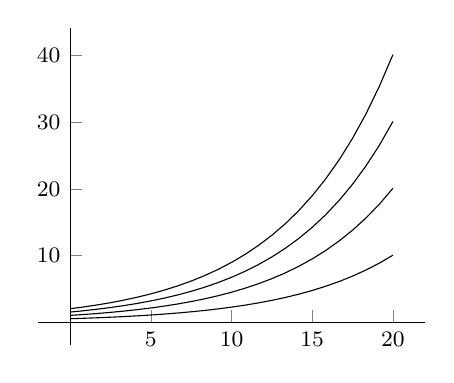
\begin{tikzpicture}
\begin{axis}[small,axis lines*=middle,ylabel style={rotate=-90},ylabel style={at={(axis description cs:0,1.05)}}]
\addplot[domain=0:20]{2*e^(0.15*x)};
\addplot[domain=0:20]{1.5*e^(0.15*x)};
\addplot[domain=0:20]{1*e^(0.15*x)};
\addplot[domain=0:20]{0.5*e^(0.15*x)};
\end{axis}
\end{tikzpicture}
\caption*{(الف) قوت نمائی اضافہ۔مساوات \عددی{y'=0.15y} کا حل۔}
\end{subfigure}%
\begin{subfigure}{0.5\textwidth}
\centering
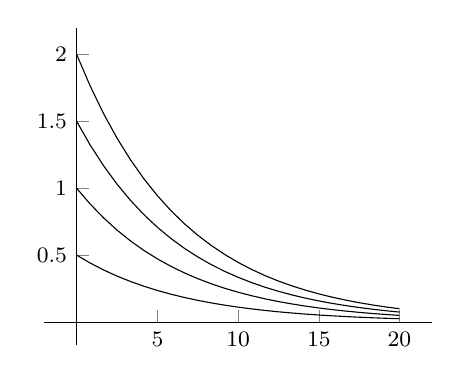
\begin{tikzpicture}
\begin{axis}[small,axis lines*=middle,ylabel style={rotate=-90},ylabel style={at={(axis description cs:0,1.05)}}]
\addplot[domain=0:20]{2*e^(-0.15*x)};
\addplot[domain=0:20]{1.5*e^(-0.15*x)};
\addplot[domain=0:20]{1*e^(-0.15*x)};
\addplot[domain=0:20]{0.5*e^(-0.15*x)};
\end{axis}
\end{tikzpicture}
\caption*{(الف) قوت نمائی گھٹاو۔مساوات \عددی{y'=-0.15y} کا حل۔}
\end{subfigure}%
\caption{قوت نمائی تفرقی مساوات کی نسل حل۔}
\label{شکل_مثال_تفرقی_اول_مالتُھس_الف}
\end{figure}
\انتہا{مثال}
%==========================

درج بالا مثالوں میں ہم نے دیکھا کہ درجہ اول سادہ تفرقی مساوات کے حل میں ایک عدد اختیاری مستقل \عددی{c} پایا جاتا ہے۔ تفرقی مساوات کا ایسا حل جس میں اختیاری مستقل \عددی{c} پایا جاتا ہو \اصطلاح{عمومی حل}\فرہنگ{عمومی حل}\فرہنگ{حل!عمومی}\حاشیہب{general solution}\فرہنگ{general solution} کہلاتا ہے۔

(بعض اوقات \عددی{c} مکمل طور اختیاری مستقل نہیں ہوتا بلکہ اس کی قیمت کو کسی وقفے پر محدود کرنا لازم ہوتا ہے۔)

ہم \اصطلاح{یکتا}\فرہنگ{یکتا!حل}\حاشیہب{unique}\فرہنگ{unique!general solution} عمومی حل حاصل کرنے کی تراکیب سیکھیں گے۔

جیومیٹریائی طور پر سادہ تفرقی مساوات کا عمومی حل لامتناہی حل کے خطوط پر مشتمل ہوتا ہے جہاں \عددی{c} کی ہر انفرادی قیمت منفرد خط دیتی ہے۔عمومی حل میں \عددی{c} کی کوئی مخصوص قیمت مثلاً \عددی{c=-3.501} یا \عددی{c=0} پر کرنے سے ہمیں \اصطلاح{جبری حل}\فرہنگ{جبری!حل}\فرہنگ{حل!جبری}\حاشیہب{particular solution}\فرہنگ{solution!particular} ملتا ہے۔جبری حل میں کوئی اختیاری مستقل نہیں پایا جاتا۔

عام طور عمومی حل قابل حصول ہوتا ہے جس میں \عددی{c} کی مخصوص قیمت پر کرتے ہوئے درکار جبری حل حاصل کیا جا سکتا ہے۔بعض اوقات تفرقی مساوات ایسا حل بھی رکھتا ہے جس کو عمومی حل سے حاصل نہیں کیا جا سکتا۔ایسے حل کو \اصطلاح{نادر}\فرہنگ{نادر!حل}\فرہنگ{حل!نادر}\حاشیہب{singular solution}\فرہنگ{singular!solution} حل کہتے ہیں۔صفحہ \حوالہصفحہ{سوال_سادہ_اول_نادر_حل_الف} پر سوال \حوالہ{سوال_سادہ_اول_نادر_حل_الف} میں نادر حل کی مثال دی گئی ہے۔

\جزوحصہء{ابتدائی قیمت سوال}
عام طور پر عمومی حل میں \اصطلاح{ابتدائی قیمتیں}\فرہنگ{ابتدائی قیمتیں}\حاشیہب{initial values}\فرہنگ{initial values} \عددی{x_0} اور \عددیء{y_0} پر کرنے سے جبری حل حاصل کیا جاتا ہے جہاں  \عددی{{y(x_0)=y_0}}  ہے۔جیومیٹریائی طور پر اس کا مطلب ہے کہ خط حل نقطہ \عددی{(x_0,y_0)} سے گزرتا ہے۔سادہ تفرقی مساوات اور مساوات کے ابتدائی قیمتوں کو \اصطلاح{ابتدائی قیمت سوال}\فرہنگ{ابتدائی قیمت سوال}\حاشیہب{initial value problem}\فرہنگ{initial value!problem} کہا جاتا ہے۔یوں صریح سادہ تفرقی مساوات کی صورت میں ابتدائی قیمت سوال درج ذیل لکھا جائے گا۔
\begin{align}
y'=f(x,y), \quad \quad y(x_0)=y_0
\end{align}

%======================
\ابتدا{مثال}
ابتدائی قیمت سوال: درج ذیل ابتدائی قیمت سوال کو حل کریں۔
\begin{align*}
y'=5y,\quad \quad y(0)=3.2
\end{align*}

حل:تفرقی مساوات کو \عددی{\tfrac{\dif y}{y}=5 \dif x} لکھتے ہوئے دونوں اطراف کا تکمل لینے سے \عددی{y=ce^{5x}} عمومی حل حاصل ہوتا ہے جس میں \عددی{x=0} پر \عددی{y=3.2} پر کرنے سے \عددی{y(0)=ce^{0}=3.2} لکھا جائے گا جس سے \عددی{c=3.2} ملتا ہے۔یوں ابتدائی قیمت سوال کا جبری حل \عددی{y=3.2e^{5x}} ہے۔
\انتہا{مثال}

%=============================
\جزوحصہء{نمونہ کشی پر مزید بحث}
نمونہ کشی کو مثال کی مدد سے بہتر سمجھا جا سکتا ہے لہٰذا ایسا ہی کرتے ہیں۔ایسا کرتے ہوئے پہلی قدم پر  مسئلے کو تفرقی مساوات کا جامہ پہنایا جائے گا۔دوسری قدم پر تفرقی مساوات کا عمومی حل حاصل کیا جائے گا۔تیسرے قدم پر ابتدائی معلومات استعمال کرتے ہوئے جبری حل حاصل کیا جائے گا۔ آخر میں چوتھا قدم حاصل جواب کی تشریح ہو گی۔ 
%=================

\ابتدا{مثال}\شناخت{مثال_اول_سادہ_تابکاری_الف}
تابکار  مادے کی موجودہ کمیت \عددی{\SI{2}{\milli\gram}} ہے۔اس کی کمیت  مستقبل میں دریافت کریں۔

طبعی معلومات: تجربے سے معلوم کیا گیا ہے کہ کسی بھی لمحے پر تابکاری تحلیل کی شرح اس لمحے پر موجود تابکار مادے کی کمیت کے راست تناسب ہے۔ 
\begin{itemize}
\item
پہلا قدم: مسئلے کو مساوات کی صورت میں لکھتے ہیں۔کمیت کو \عددی{y} سے ظاہر کرتے ہیں۔یوں کسی بھی لمحے پر تابکاری کی شرح سے مراد \عددی{y'=\tfrac{\dif y}{\dif t}} ہے جہاں \عددی{t} وقت کو ظاہر کرتا ہے۔چونکہ تابکاری سے تابکار مادے کی کمیت گھٹتی ہے لہٰذا تجربے سے حاصل معلومات کو درج ذیل تفرقی مساوات کی صورت میں لکھا جائے گا جہاں تناسبی مستقل \عددی{k} مثبت قیمت ہے۔
\begin{align}
\frac{\dif y}{\dif t}=-ky
\end{align}
مثال \حوالہ{مثال_تفرقی_اول_مالتھس_الف} میں آپ نے دیکھا کہ تفرقی مساوات میں منفی کی علامت سے تفرقی مساوات کا قوت نمائی گھٹتا ہوا حل حاصل ہوتا ہے۔چونکہ تابکاری سے تابکار مادے کی کمیت گھٹتی ہے لہٰذا درج بالا مساوات میں منفی کی علامت استعمال کی گئی ہے۔تابکار اشیاء کے مستقل \عددی{k} کی قیمتیں تجربے سے حاصل کئے جاتے ہیں مثلاً \اصطلاح{ریڈیم}\فرہنگ{ریڈیم}\حاشیہب{radium}\فرہنگ{radium} یعنی   \عددی{\ce{^{226}_{88}Ra}} کا \عددی{k=\SI{1.4e-11}{\per\second}} ہے۔

ابتدائی کمیت \عددی{\SI{2}{\milli\gram}} ہے۔ابتدائی وقت کو \عددی{t=0} لیتے  ہوئے ابتدائی معلومات \عددی{y(0)=\SI{2}{\milli\gram}} لکھی  جائے گی۔(غیر تابع متغیر وقت \عددی{t} کی بجائے  کچھ اور مثلاً \عددی{x} ہونے کی صورت میں بھی \عددی{(x_0,y_0)} یا \عددی{y(x_0)=y_0} کو ابتدائی معلومات ہی کہا جاتا ہے۔اسی طرح تابع متغیرہ \عددی{y} کی قیمت \عددی{t \ne 0} پر معلوم ہو سکتی ہے مثلاً \عددی{y(x_n)=y_n} اور ایسی صورت میں \عددی{(x_n,y_n)} ابتدائی معلومات کہلاتی ہے۔یوں دیے مسئلے سے درج ذیل ابتدائی قیمت سوال حاصل ہوتا ہے۔
\begin{align}
y'=-ky,\quad \quad y(0)=\SI{2}{\milli\gram} 
\end{align}

\item
دوسرا قدم:ابتدائی قیمت سوال کا عمومی حل درج ذیل ہے جہاں \عددی{c} اختیاری مستقل جبکہ \عددی{k} کی قیمت تابکار مادے پر منحصر ہے۔
\begin{align}
y=c^{-kt}
\end{align}
ابتدائی معلومات کے تحت \عددی{t=0} پر \عددی{y=\SI{2}{\milli\gram}} ہے جس کو درج بالا مساوات میں پر کرتے ہوئے \عددی{c=2} حاصل ہوتا ہے۔یوں درج ذیل جبری حل حاصل ہوتا ہے۔
\begin{align}\label{مساوات_سادہ_اول_جبری_تابکاری}
y=2e^{-kt}\quad \quad (k>0)
\end{align} 
جبری حل کو واپس تفرقی مساوات میں پر کرتے ہوئے ثابت کریں کہ حاصل حل درست ہے۔اسی طرح جبری حل سے ابتدائی معلومات حاصل کریں۔
\begin{align*}
\frac{\dif y}{\dif t}=-k ce^{-kt}=-ky\\
y(0)=2e^{-0}=2
\end{align*}
%
\item
حاصل جبری حل کی تشریح:مساوات \حوالہ{مساوات_سادہ_اول_جبری_تابکاری} کو شکل \حوالہ{شکل_مثال_اول_سادہ_تابکاری_الف} میں دکھایا گیا ہے جہاں \عددی{k=2.5} لیا گیا ہے۔لمحہ \عددی{t=0} پر یہ مساوات تابکار مادے کی درست کمیت دیتا ہے۔لمحہ لامتناہی پر تابکار مادے کی کمیت \عددی{y(\infty)=2e^{-k\infty}=0} حاصل ہوتی ہے۔
\begin{figure}
\centering
\begin{tikzpicture}
\begin{axis}[small,axis lines*=middle,ylabel style={rotate=-90},ylabel style={at={(axis description cs:0,1.05)}},xlabel={$t$},ylabel={$y$}]
\addplot[domain=0:2]{2*e^(-2.5*x)};
\end{axis}
\end{tikzpicture}
\caption{مثال \حوالہ{مثال_اول_سادہ_تابکاری_الف} کی منحنی۔ تابکاری تحلیل \عددی{y=2e^{-kt}} جہاں \عددی{k=2.5} لیا گیا ہے۔}
\label{شکل_مثال_اول_سادہ_تابکاری_الف}
\end{figure} 
%
\end{itemize}
\انتہا{مثال}
%=====================
سوالات \حوالہ{سوال_سادہ_اول_تکمل_الف} تا \حوالہ{سوال_سادہ_اول_تکمل_آخر} کے جوابات بذریعہ تکمل حاصل کریں یا کسی تفاعل کی تفرق سے جواب حاصل کریں۔

\ابتدا{سوال}\شناخت{سوال_سادہ_اول_تکمل_الف}
\quad
$y'+3\sin 2\pi x=0$

جواب:\quad
  $y=\frac{3}{2\pi} \cos 2\pi x+c$
\انتہا{سوال}
%=====================
\ابتدا{سوال}\quad
$y'+xe^{-x^2}=0$

جواب:\quad
$y=\tfrac{e^{-x^2}}{2}+c$
\انتہا{سوال}
%==================
\ابتدا{سوال}\quad
$y'=4e^{-x}\cos x$

جواب:\quad
 $y=2e^{-x}(\cos x-\sin x)+c$
\انتہا{سوال}
%=======================
\ابتدا{سوال}\quad
$y'=y$

جواب:\quad
$y=ce^{x}$
\انتہا{سوال}
%======================
\ابتدا{سوال}\quad
$y'=-y$

جواب:\quad
$y=ce^{-x}$
\انتہا{سوال}
%======================
\ابتدا{سوال}\quad
$y'=2.2y$

جواب:\quad
$y=ce^{2.2x}$
\انتہا{سوال}
%======================
\ابتدا{سوال}\quad
$y'=1.5\sinh 3.2x$

جواب:\quad
$y=\tfrac{15}{32}\cosh 3.2x+c$
\انتہا{سوال}
%======================
\ابتدا{سوال}\شناخت{سوال_سادہ_اول_تکمل_آخر}
\quad
$y''=-y$

جواب:\quad
$y=c_1\cos x+c_2\sin x$
\انتہا{سوال}
%======================
سوال \حوالہ{سادہ_اول_ابتدائی_قیمت_الف} تا سوال \حوالہ{سادہ_اول_ابتدائی_قیمت_آخر} ابتدائی قیمت سوالات ہیں جن کے عمومی حل دیے گئے ہیں۔انہیں تفرقی مساوات میں پر کرتے ہوئے ثابت کریں کہ یہی عمومی جوابات ہیں۔عمومی جواب سے جبری جواب حاصل کریں۔جبری جواب کا خط کھینچیں۔

%=================================
\ابتدا{سوال}\شناخت{سادہ_اول_ابتدائی_قیمت_الف}
\quad
$y'+2y=0.8,\quad y=ce^{-2x}+0.4,\quad y(0)=1.2$

جواب:\quad
$y=0.8e^{-2x}+0.4$
\انتہا{سوال}
%==========================
\ابتدا{سوال}\quad
$y'+x+y=0,\quad y=ce^{-x}-x+1,\quad y(0)=\pi$

جواب:\quad
$y=\pi e^{-x}-e^{-x}-x+1$
\انتہا{سوال}
%==========================
\ابتدا{سوال}\quad
$y'=2x+e^{x},\quad y=e^{x}+x^2+c,\quad y(0)=1$

جواب:\quad
$y=e^{x}+x^2$
\انتہا{سوال}
%==================
\ابتدا{سوال}\quad
$y'+4xy=0,\quad y=ce^{-2x^2},\quad y(0)=2$

جواب:\quad
$y=2e^{-2x^2}$
\انتہا{سوال}
%==========
\ابتدا{سوال}\quad
$yy'=2x,\quad y^2=2x^2+c,\quad y(1)=6$

جواب:\quad
$y^2=2x^2+34$
\انتہا{سوال}
%======================
\ابتدا{سوال}\quad
$y'=y+y^2,\quad y=\tfrac{c}{e^{-x}-c},\quad y(0)=0.1$

جواب:\quad
$y=\tfrac{1}{e^{(-x+23.98)}-1}$
\انتہا{سوال}
%==================
\ابتدا{سوال}\شناخت{سادہ_اول_ابتدائی_قیمت_آخر}
\quad
$y'\tan x=y-4,\quad y=c\sin x+4,\quad y(\tfrac{\pi}{2})=0$

جواب:\quad
$y=4-4\sin x$
\انتہا{سوال}
%================
\ابتدا{سوال}\شناخت{سوال_سادہ_اول_نادر_حل_الف}
نادر حل: بعغ اوقات سادہ تفرقی مساوات کا ایسا حل بھی پایا جاتا ہے جس کو عمومی حل سے حاصل نہیں کیا جا سکتا۔ایسیے حل کو \اصطلاح{نادر حل}\فرہنگ{نادر!حل}\فرہنگ{حل!نادر}\حاشیہب{singular solution}\فرہنگ{solution!singular} کہا جاتا ہے۔مساوات \عددی{y'^2-xy'+y=0} کا عمومی حل \عددی{y=cx-c^{2}} ہے جبکہ اس کا  نادر حل \عددی{y=\tfrac{x^2}{4}} ہے۔ ان حل کا تفرق لیتے ہوئے تفرقی مساوات میں پر کرتے ہوئے ثابت کریں کہ یہ تفرقی مساوات کے حل ہیں۔
\انتہا{سوال}
%=================
سوال \حوالہ{سوال_سادہ_اول_نقشہ_کشی_الف} تا سوال \حوالہ{سوال_سادہ_اول_نقشہ_کشی_ٹ} نقشہ کشی کے سوالات ہیں۔

\ابتدا{سوال}\شناخت{سوال_سادہ_اول_نقشہ_کشی_الف}
تابکار مادے کی نصف زندگی \عددی{t_{\tfrac{1}{2}}} سے مراد وہ دورانیہ ہے جس میں تابکار مادے کی کمیت نصف ہو جاتی ہے۔مثال \حوالہ{مثال_اول_سادہ_تابکاری_الف} میں ریڈیم \ce{^{266}_{88}Ra} کی نصف زندگی دریافت کریں۔

جواب:تابکاری تحلیل کی مساوات \عددی{y=y_0e^{-kt}} میں لمحہ \عددی{t=0} پر (ابتدائی) کمیت\عددی{y_0} ہے جبکہ مستقبل میں لمحہ \عددی{t} پر کمیت \عددی{y} ہے۔ہم وہ دورانیہ جاننا چاہتے ہیں جس میں کمیت نصف رہ جائے یعنی جب \عددی{y=\tfrac{y_0}{2}} رہ جائے۔تابکاری مساوات میں \عددی{y=\tfrac{y_0}{2}} پر کرتے ہوئے \عددی{\tfrac{y_0}{2}=y_0e^{-kt}} لکھا جائے گا جس سے \عددی{t_{\tfrac{1}{2}}=\SI{4.95e10}{\second}}  یعنی \عددی{1569.6} سال  حاصل ہوتا ہے۔یوں ریڈیم کی مقدار \عددی{1569.6} سالوں میں نصف رہ جائے گی۔ 
\انتہا{سوال}
%==============================
\ابتدا{سوال}\شناخت{سوال_سادہ_اول_نقشہ_کشی_ب}
ریڈیم \اصطلاح{ہم جا}\فرہنگ{ہم جا}\حاشیہب{isotope}\فرہنگ{isotope} \ce{^{224}_{88}Ra} کی نصف زندگی تقریباً \عددی{3.6} دن ہے۔دو گرام \عددیء{(\SI{2}{\gram})} ریڈیم ہم جا کی کمیت ایک دن بعد کتنی رہ جائے گی۔دو گرام ریڈیم ہم جا کی کمیت ایک سال بعد کتنی رہ جائے گی۔

جوابات:\عددی{\SI{1.65}{\gram}}، \عددی{\SI{6e-31}{\gram}}
\انتہا{سوال}
%======================
\ابتدا{سوال}\شناخت{سوال_سادہ_اول_نقشہ_کشی_پ}
ایک جہاز کی رفتار مستقل اسراع \عددی{a} سے مسلسل بڑھ رہی ہے۔رفتار کی تبدیلی کی شرح \عددی{\tfrac{\dif v}{\dif t}} کو اسراع کہتے ہیں۔ان معلومات سے تفرقی مساوات لکھتے ہوئے لمحہ \عددی{t} پر رفتار \عددی{v} کی مساوات حاصل کریں۔اگر \عددی{t=0} پر ابتدائی رفتار \عددی{u} ہو تب \عددی{v} کی مساوات کیا ہو گی؟ 

جوابات:\عددی{v=at+c}، \عددی{v=u+at}
\انتہا{سوال}
%=========================
\ابتدا{سوال}\شناخت{سوال_سادہ_اول_نقشہ_کشی_ت}
رفتار سے مراد وقت کے ساتھ فاصلے کی تبدیلی کی شرح \عددی{\tfrac{\dif x}{\dif t}} ہے۔سوال \حوالہ{سوال_سادہ_اول_نقشہ_کشی_پ} میں رفتار کی مساوات \عددی{v=u+at} حاصل کی گئی جسے \عددی{\tfrac{\dif x}{\dif t}} کے برابر پر کرنے سے تفرقی مساوات حاصل ہوتی ہے۔لمحہ \عددی{t=0} پر ابتدائی فاصلہ \عددی{x=0} لیتے ہوئے ابتدائی قیمت سوال کو حل کرتے ہوئے  \عددی{x} کی مساوات حاصل کریں۔

جوابات:\عددی{x=ut+\tfrac{1}{2}at^2}
\انتہا{سوال}
%=========================
\ابتدا{سوال}\شناخت{سوال_سادہ_اول_نقشہ_کشی_ٹ}
آواز سے کم رفتار پر پرواز کرنے والے جہاز کی کارگزاری ہوا کے دباو پر منحصر ہوتی ہے۔ان  کی کارگزاری \عددی{\SI{10500}{\meter}} تا \عددی{\SI{12000}{\meter}} کی اونچائی پر بہترین حاصل ہوتی ہے۔آپ سے گزارش ہے کہ \عددی{\SI{10500}{\meter}} کی اونچائی پر ہوا کا دباو دریافت کریں۔طبعی معلومات:اونچائی کے ساتھ دباو میں تبدیلی کی شرح \عددی{y'} ہوا کے دباو \عددی{y} کے راست تناسب ہوتی ہے۔تقریباً \عددی{\SI{5500}{\meter}} کی اونچائی پر ہوا کا دباو سمندر کی سطح پر ہوا کے دباو \عددی{y_0} کی نصف ہوتا ہے۔

جواب:\عددی{0.27y_0}یعنی تقریباً ایک چوتھائی
\انتہا{سوال}
%===================

\حصہ{\عددی{y'=f(x,y)} کا جیومیٹریائی مطلب۔ میدان کی سمت اور ترکیب یولر۔}
درجہ اول سادہ تفرقی مساوات
\begin{align}\label{مساوات_سادہ_اول_ڈھلوان_تفاعل_الف}
y'=f(x,y)
\end{align}
سادہ معنی رکھتی ہے۔آپ جانتے ہیں کہ \عددی{y'} سے مراد \عددی{y} کی ڈھلوان ہے۔یوں مساوات \حوالہ{مساوات_سادہ_اول_ڈھلوان_تفاعل_الف} کا وہ حل جو نقطہ \عددی{(x_0,y_0)} سے گزرتا ہو کا اس نقطے پر ڈھلوان \عددی{y'(x_0)} ہو گا کو درج بالا مساوات کے تحت اس نقطے پر \عددی{f} کی قیمت کے برابر ہو گا۔
\begin{align*}
y'(x_0)=f(x_0,y_0)
\end{align*}
اس حقیقت کو استعمال کرتے ہوئے ہم مساوات \حوالہ{مساوات_سادہ_اول_ڈھلوان_تفاعل_الف} کو حل کرنے کے  \اصطلاح{ترسیمی}\فرہنگ{ترسیمی}\حاشیہب{graphical}\فرہنگ{graphical} یا \اصطلاح{اعدادی}\فرہنگ{اعدادی}\حاشیہب{numerical}\فرہنگ{numerical} طریقے دریافت کر سکتے ہیں۔تفرقی مساوات کو حل کرنے کے ترسیمی اور اعدادی طریقے اس لئے بھی اہم ہیں کہ کئی تفرقی مساوات کا کوئی \اصطلاح{تحلیلی}\فرہنگ{تحلیلی}\حاشیہب{analytic}\فرہنگ{analytic} حل نہیں پایا جاتا جبکہ ہر قسم کے تفرقی مساوات کا ترسیمی اور اعدادی حل حاصل کرنا ممکن ہے۔   

\جزوحصہء{میدان کی سمت: ترسیمی طریقہ}
ہم \عددی{xy} سطح پر جگہ جگہ مساوات \حوالہ{مساوات_سادہ_اول_ڈھلوان_تفاعل_الف} سے حاصل ڈھلوان کی چھوٹی لمبائی کی سیدھی لکیریں کھینچ سکتے ہیں۔ہر نقطے پر ایسی لکیر اس نقطے پر میدان کی سمت دیتی ہے۔اس \اصطلاح{میدانِ سمت}\فرہنگ{میدانِ!سمت}\حاشیہب{direction field}\فرہنگ{direction field} یا  \اصطلاح{میدانِ ڈھال}\فرہنگ{میدان!ڈھال}\فرہنگ{ڈھال!میدان}\حاشیہب{slope field}\فرہنگ{field!slope}\فرہنگ{slope!field} میں تفرقی مساوات کا  \اصطلاح{منحنی حل}\فرہنگ{منحنی حل}\حاشیہب{solution curve}\فرہنگ{solution curve} کھینچا جا سکتا ہے۔

منحنی حل کو کھینچنے کی ترکیب کچھ یوں ہے۔کسی بھی نقطے پر ڈھلوان کی سمت میں چھوٹی لکیر کھینچیں۔اس لکیر کو آہستہ آہستہ یوں موڑیں کہ لکیر کے اختتامی نقطے پر لکیر کی ڈھلوان عین اس نقطے کی ڈھلوان برابر ہو۔اسی طرح آگے بڑھتے رہیں۔ڈھال میدان میں نقطے جتنے قریب قریب ہوں تفرقی مساوات کا منحنی حل اتنا درست ہو گا۔

شکل \حوالہ{شکل_اول_سادہ_منحنی_حل_الف} میں 
\begin{align}\label{مساوات_اول_سادہ_ب}
y=x-y
\end{align}
کا ڈھال میدان دکھایا گیا ہے۔ساتھ ہی ساتھ چند منحنی حل بھی دکھائے گئے ہیں۔
\begin{figure}
\centering
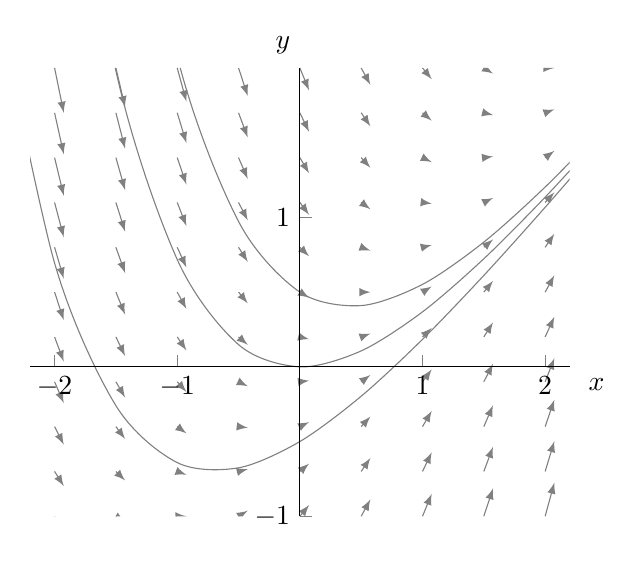
\begin{tikzpicture}
\begin{axis}[ axis lines*=middle,view={0}{90}, xlabel={$x$},ylabel={$y$},ylabel style={rotate=-90},ylabel style={at={(axis description cs:0.5,1.05)}},xmin=-2.2, xmax=2.2, ymin=-1, ymax=2,domain=-2.5:2.5, y domain=-1:2, samples=11,ytick={-1,0,1},yticklabels={$-1$,$0$,$1$},xlabel style={at={(axis description cs:1.05,0.33)}}]
\addplot3 [gray, quiver={u={1}, v={x-y}, scale arrows=0.075,
               every arrow/.append style={-latex}}] (x,y,0); %differential equation
\addplot [gray,smooth]{x-1+e^(-x)}; %actual curve
\addplot [gray,smooth]{x-1+0.5*e^(-x)}; %actual curve
\addplot [gray,smooth]{x-1+1.5*e^(-x)}; %actual curve
\end{axis}
\end{tikzpicture}
\caption{درجہ اول سادہ تفرقی مساوات \عددی{y'=x-y} کا ڈھال میدان اور منحنی حل۔}
\label{شکل_اول_سادہ_منحنی_حل_الف}
\end{figure}

آئیں اب اعدادی طریقہ سیکھیں۔سادہ ترین اعدادی طریقہ \اصطلاح{ترکیب یولر} کہلاتا ہے۔پہلے اسی پر بحث کرتے ہیں۔

\جزوحصہء{یولر کی اعدادی ترکیب}
درجہ اول تفرقی مساوات \عددی{y'=f(x,y)} اور ابتدائی معلومات \عددی{y(x_0)=y_0} کو استعمال کرتے ہوئے  \اصطلاح{ترکیب یولر}\فرہنگ{یولر!ترکیب}\حاشیہب{Euler's method}\فرہنگ{Euler's method} ہم فاصلہ نقطوں \عددی{x_0}، \عددی{x_1=x_0+h}، \عددی{x_2=x_0+2h}، \عددی{\cdots} پر تقریباً درست قیمتیں دیتا ہے یعنی
\begin{align*}
y_1&=y_0+hf(x_0,y_0)\\
y_2&=y_1+hf(x_1,y_1)\\
y_3&=y_2+hf(x_2,y_2)
\end{align*}
یا
\begin{align}
y_{n+1}=y_n+hf(x_n,y_n)
\end{align}
جہاں \عددی{h} کی قیمت جتنی کم ہو، حاصل حل اتنا بہتر ہو گا۔

آئیں اب \عددی{h=0.1} لیتے ہوئے  مساوات \حوالہ{مساوات_اول_سادہ_ب} کو ترکیب یولر سے حل کریں۔
